\chapter{The Verified Symbolic Compute Pipeline: Overview}
\label{ch:vscp}

\section{Safety Boundaries as a Design Discipline}
\label{sec:vscp-boundary}

The pipeline is best understood as a sequence of boundaries, not a sequence
of transforms. A \emph{boundary} has three parts:
\begin{enumerate}
  \item an \textbf{inbound contract} (what the previous layer promised),
  \item a \textbf{transformation} (what this layer does), and
  \item an \textbf{outbound contract} (what the next layer may assume).
\end{enumerate}
If the inbound contract is violated, the layer must fail loudly and seal a
receipt recording the failure. If the transformation succeeds, the outbound
contract is certified. This discipline is what makes the system
\emph{inspectable}: any artifact can be traced to the exact boundary that
produced it and the exact receipt that certified it.

\section{Data Flow}
\label{sec:vscp-flow}

\begin{figure}[H]
\centering
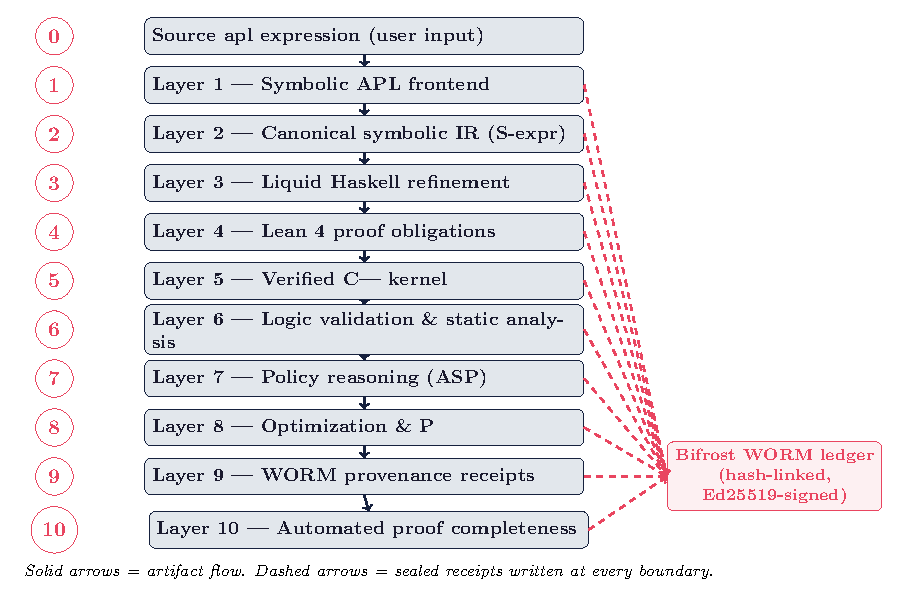
\includegraphics[width=\textwidth]{figs/vscp_layers.pdf}
\caption{The ten safety boundaries and their artifact types. Dashed arrows
denote sealed receipts written to the WORM ledger (Layer~9).}
\label{fig:vscp}
\end{figure}

The end-to-end flow for the sum-of-squares example is:
\begin{enumerate}
  \item \textbf{L1 (APL)}: \texttt{SumSquares <- { (+/ (\ensuremath{iota}\ensuremath{omega}) * 2) }}.
  \item \textbf{L2 (IR)}: parse to a typed AST, normalize to canonical
        S-expression.
  \item \textbf{L3 (Liquid)}: refine the AST (well-formedness, degree bounds).
  \item \textbf{L4 (Lean)}: emit \texttt{theorem} obligations; prove or
        \texttt{sorry}.
  \item \textbf{L5 (C{--})}: compute the closed form in the verified kernel.
  \item \textbf{L6 (Logic/Static)}: FOL consistency + CodeQL checks.
  \item \textbf{L7 (ASP)}: policy allows publication.
  \item \textbf{L8 (Opt/PNP)}: seal skill; optional swarm search for harder
        cases.
  \item \textbf{L9 (WORM)}: every artifact above is receipted and signed.
  \item \textbf{L10 (Completeness)}: \texttt{sorryhunter} attempts to close
        remaining gaps; \texttt{sorrydb} records status.
\end{enumerate}

\section{Why Ten Layers and Not Fewer}
\label{sec:vscp-why}

Each layer answers a distinct question:
\begin{itemize}
  \item L1: \emph{What did the user mean?} (notation $\ensuremath{rightarrow}$ AST)
  \item L2: \emph{What is the canonical form?} (normalization)
  \item L3: \emph{Is it structurally sound?} (refinement)
  \item L4: \emph{Can it be proven?} (obligations)
  \item L5: \emph{Does it compute correctly?} (verified kernel)
  \item L6: \emph{Is the logic and code safe?} (analysis)
  \item L7: \emph{Is it permitted?} (policy)
  \item L8: \emph{Can it be improved/found?} (optimization/search)
  \item L9: \emph{Who/what produced it, and when?} (provenance)
  \item L10: \emph{Is the proof complete?} (closure)
\end{itemize}
Collapsing layers would merge incompatible contracts and hide the point of
failure. The cost of ten layers is verbosity; the benefit is that a wrong
result is always attributable to one boundary.

\section{The Reference Implementation Map}
\label{sec:vscp-map}

Table~\ref{tab:impl-map} maps each layer to its concrete artifacts in the
repository. Subsequent chapters expand each row.

\begin{table}[H]
\centering
\caption{Layer $\ensuremath{rightarrow}$ implementation map.}
\label{tab:impl-map}
\begin{tabularx}{\textwidth}{clX}
\toprule
\textbf{\#} & \textbf{Path} & \textbf{Key files} \\
\midrule
1  & \texttt{layers/apl/}        & \texttt{src/Parser.hs} \\
2  & \texttt{layers/sexpr/}      & \texttt{src/AST.hs} \\
3  & \texttt{layers/liquid/}     & \texttt{src/Bridge.hs} \\
4  & \texttt{layers/hol/lean/}   & \texttt{Mathlib5/Core.lean} \\
5  & \texttt{kernel/}            & \texttt{verified\_kernel.cm} \\
6  & \texttt{layers/fol/}, \texttt{layers/codeql/} & resolution checker, static analysis \\
7  & \texttt{layers/asp/}        & stable models (Clingo) \\
8  & \texttt{layers/prism-skills/}, \texttt{layers/pnp-attack/} & canonical JSON, swarm \\
9  & \texttt{(receipts)}         & \texttt{scripts/receipt.sh} \\
10 & \texttt{layers/sorryhunter/}, \texttt{sorrydb/} & closure engine, ledger \\
\bottomrule
\end{tabularx}
\end{table}
